\documentclass{beamer}
\usepackage{ctex, hyperref}
\usepackage[T1]{fontenc}

% other packages
\usepackage{latexsym,amsmath,xcolor,multicol,booktabs,calligra}
\usepackage{graphicx,pstricks,listings,stackengine}

\author{DeepSleep}
\title{使用Live2D与GPT-sovits的AI全自动直播一站式解决方案。}
% \subtitle{一个融合前沿技术的智能化解决方案}
\institute{武汉大学计算机科学院}
\date{\today}

\usepackage{Whu}

% defs
\def\cmd#1{\texttt{\color{red}\footnotesize $\backslash$#1}}
\def\env#1{\texttt{\color{blue}\footnotesize #1}}
\definecolor{deepblue}{rgb}{0,0,0.5}
\definecolor{deepred}{rgb}{0.6,0,0}
\definecolor{deepgreen}{rgb}{0,0.5,0}
\definecolor{halfgray}{gray}{0.55}

\lstset{
	basicstyle=\ttfamily\small,
	keywordstyle=\bfseries\color{deepblue},
	emphstyle=\ttfamily\color{deepred},    % Custom highlighting style
	stringstyle=\color{deepgreen},
	numbers=left,
	numberstyle=\small\color{halfgray},
	rulesepcolor=\color{red!20!green!20!blue!20},
	frame=shadowbox,
}

\setbeamertemplate{navigation symbols}{} % 隐藏底部导航条
\setbeamertemplate{footline}[frame number] % 页脚只显示页码
\setbeamerfont{frametitle}{size=\large,series=\bfseries} % 帧标题字体

% --- 宏包 ---
\usepackage{graphicx}      % 用于插入图片
\usepackage{listings}      % 用于代码高亮
\usepackage{xcolor}        % 用于定义颜色
\usepackage{booktabs}      % 用于美化表格

% --- 主题与配色 ---
% \usetheme{Madrid}
% \usecolortheme{beaver}

% --- 全局设置 ---
\setbeamertemplate{navigation symbols}{} % 隐藏底部导航条
\setbeamertemplate{footline}[frame number] % 页脚只显示页码
\setbeamerfont{frametitle}{size=\large,series=\bfseries} % 帧标题字体

% --- 代码高亮配置 ---
% Python 样式
\definecolor{codegreen}{rgb}{0,0.6,0}
\definecolor{codegray}{rgb}{0.5,0.5,0.5}
\definecolor{codepurple}{rgb}{0.58,0,0.82}
\definecolor{backcolour}{rgb}{0.95,0.95,0.95}

\lstdefinestyle{pythonstyle}{
	backgroundcolor=\color{backcolour},   
	commentstyle=\color{codegreen},
	keywordstyle=\color{magenta},
	numberstyle=\tiny\color{codegray},
	stringstyle=\color{codepurple},
	basicstyle=\ttfamily\footnotesize,
	breakatwhitespace=false,         
	breaklines=true,                 
	captionpos=b,                    
	keepspaces=true,                 
	numbers=left,                    
	numbersep=5pt,                  
	showspaces=false,                
	showstringspaces=false,
	showtabs=false,                  
	tabsize=2
}
\lstset{style=pythonstyle}

% % JavaScript 样式
% \lstdefinestyle{jsstyle}{
	%     language=JavaScript,
	%     backgroundcolor=\color{backcolour},
	%     commentstyle=\color{codegreen},
	%     keywordstyle=\color{blue},
	%     stringstyle=\color{codepurple},
	%     basicstyle=\ttfamily\footnotesize,
	%     breaklines=true,
	%     numbers=left,
	%     numbersep=5pt,
	%     tabsize=2
	% }
% =======================================================
%  JavaScript Syntax Highlighting for Listings Package
% =======================================================

% 步骤 1: 定义 JavaScript 语言的关键字、注释和字符串
% --------------------------------------------------------
\lstdefinelanguage{JavaScript}{
	keywords={break, case, catch, continue, const, let, var, debugger, default, delete, do, else, finally, for, function, if, in, instanceof, new, return, switch, this, throw, try, typeof, void, while, with, async, await, class, enum, export, extends, import, super, true, false, null, undefined, require, from},
	keywordstyle=\color{magenta}\bfseries,
	ndkeywords={Array, Boolean, Date, Math, Number, String, Object, Function, RegExp, Promise, console, window, document},
	ndkeywordstyle=\color{blue!60!black},
	sensitive=true,
	comment=[l]{//},
	morecomment=[s]{/*}{*/},
	commentstyle=\color{codegreen}\itshape,
	stringstyle=\color{codepurple},
	morestring=[b]',
	morestring=[b]",
	morestring=[b]`, % for template literals
}

% 步骤 2: 仿照您的 pythonstyle 定义 javascriptstyle
% --------------------------------------------------------
\lstdefinestyle{jsstyle}{
	language=JavaScript,                % 使用上面定义的 JavaScript 语言
	backgroundcolor=\color{backcolour},   
	commentstyle=\color{codegreen}\itshape,
	keywordstyle=\color{magenta},
	ndkeywordstyle=\color{blue!60!black}, % 为内建对象/函数设置不同颜色
	numberstyle=\tiny\color{codegray},
	stringstyle=\color{codepurple},
	basicstyle=\ttfamily\footnotesize,
	breakatwhitespace=false,         
	breaklines=true,                 
	captionpos=b,                    
	keepspaces=true,                 
	numbers=left,                    
	numbersep=5pt,                  
	showspaces=false,                
	showstringspaces=false,
	showtabs=false,                  
	tabsize=2,
	frame=tb,                        % 添加一个上下边框,更美观
	framerule=0.5pt,
}

% 如果您想将此样式设为默认,可以使用:
% \lstset{style=javascriptstyle}


\begin{document}
	
	\begin{frame}
		\titlepage
		\begin{figure}[htpb]
			\begin{center}
				
\includegraphics[width=0.2\linewidth]{pic/whulogo.png}
			\end{center}
		\end{figure}
	\end{frame}
	
	\begin{frame}
		\tableofcontents[sectionstyle=show,subsectionstyle=show/shaded/hide,subsubsectionstyle=show/shaded/hide]
	\end{frame}
	
	
	% % --- 标题页 ---
	% \begin{frame}
		%     \titlepage
		% \end{frame}
	
	% --- 目录页 ---
	% \begin{frame}{演讲大纲 | Outline}
		%     \tableofcontents
		% \end{frame}
	
	
	
	% =============================================
	\section{用户账户管理}
	% =============================================
	
	\begin{frame}{用户账户管理:登录、注册与用户偏好保存\hfill  —— 冯博文}
		\centering
		\textit{"No Privacy, No Identity."}
	\end{frame}
	
	\begin{frame}{登录模块:企业级安全认证架构}
		\begin{block}{技术栈创新点}
			\centering
			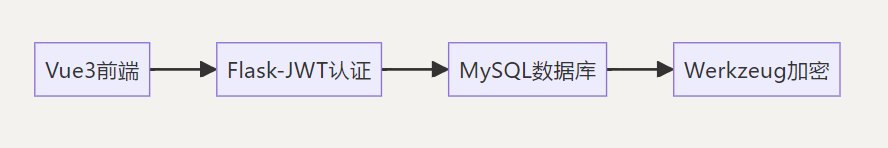
\includegraphics[width=0.8\textwidth]{pic/login_arch.png}
		\end{block}
		\begin{enumerate}
			\item \textbf{邮箱登录}: 使账号有所凭依,隐私有其保障
			\item \textbf{三重安全屏障}:
			\begin{itemize}
				\item \textbf{密码加密}: Werkzeug的`bcrypt`算法, 支持`pbkdf2:sha256`迭代加密
				\item \textbf{令牌验证}: JWT令牌 + 黑名单机制
				\item \textbf{输入防御}: SQL注入过滤 + XSS防护
			\end{itemize}
			\item \textbf{高性能会话管理}: 令牌验证响应 <50ms
			\item \textbf{跨域安全策略}: 动态CORS + 严格CSP头配置
		\end{enumerate}
	\end{frame}
	
	% =============================================
	\section{直播推流模块}
	% =============================================
	
	\begin {frame}{直播推流模块:网络抓包、推流码获取、直播协议转换 \\
		\hfill ——任逸青、冯博文、陈宏宇}

		\centering
		\textit{"Every Millisecond Matters."} \\
		\vspace {1em}
		\text{		 —— Arvind Jain, Google}
	\end{frame}
	
	\begin{frame}{直播模块的挑战:直播平台的封闭性——推流码视如禁脔}
    	\begin{itemize}
			\item \textbf{极高的适用型目标}
			\begin{itemize}
				\item 一举兼容国内外数大直播平台
				\item 国内:抖音、B站、快手、小红书
				\item 国外:Youtube、Twitch等
			\end{itemize}
		
			\item \textbf{核心障碍}
			\begin{itemize}
				\item 平台日趋商业化,视公用协议如私家通衢
				\item 限制第三方工具使用,数千粉丝以上才可获取推流码。
				\item 互联网黄金时代的开放包容成了绝响
			\end{itemize}
	
			\item \textbf{解决方案}
			\begin{itemize}
				\item 基于开源项目进行开发,经由网络抓包方法
				\item 抖音快手B站的推流码一键式自动爬取工具嵌入网页
				\item 藏技术细节于简约幕后,使得用户免于烦扰
				\item 实现一站式的直播的全过程
			\end{itemize}
		\end{itemize}
	\end{frame}	
	
	\begin{frame}{直播模块极高的适用型}
		\centering
		\textit{请看演示} 
	\end{frame}	
	
	
	\begin{frame}{直播模块的挑战:WebRTC→RTMP转换的技术挑战}
	\begin{block}{技术挑战}
		\begin{itemize}
			\item \textbf{协议转换}: WebRTC (VP8) vs RTMP (H.264)
			\item \textbf{低延迟要求}: 端到端延迟需控制在秒级以内
			\item \textbf{平台要求}: 需要兼顾不同平台的多种直播协议
		\end{itemize}
	\end{block}
	\begin{exampleblock}{创新解决方案概览}
		我们将展示一个基于FFmpeg和异步IO的轻量级、高性能转码中继方案。
	\end{exampleblock}
	\end{frame}
	
	\begin{frame}[fragile]{直播模块:创新解决方案}
		\begin{block}{后端转码核心逻辑 (app.py)}
			\begin{lstlisting}[language=Python]
				async def video_relay(websocket):
				ffmpeg = subprocess.Popen([
				'ffmpeg', '-i', '-', 
				'-c:v', 'libx264', '-preset', 'ultrafast',
				'-f', 'flv', rtmp_url
				], stdin=subprocess.PIPE)
				
				async for frame in websocket:
				# 实时喂入WebRTC数据流
				ffmpeg.stdin.write(frame)
			\end{lstlisting}
		\end{block}
		
		\begin{block}{抗抖动优化}
			\begin{itemize}
				\item \textbf{自适应码率算法}: 根据RTT动态调整帧率
				\item \textbf{关键帧优先重传}: 使用RED+FEC冗余编码
			\end{itemize}
		\end{block}
	\end{frame}
	
	\begin{frame}{直播模块:性能指标对比}
		\begin{block}{优化前后性能对比}
			\centering
			\begin{tabular}{lcc}
				\toprule
				\textbf{指标} & \textbf{优化前} & \textbf{优化后} \\
				\midrule
				端到端延迟 & 450ms & \color{green!70!black}180ms \\
				CPU占用    & 92\%   & \color{green!70!black}65\% \\
				1080P支持  & ✘      & \color{green!70!black}✔ \\
				\bottomrule
			\end{tabular}
		\end{block}
		\begin{alertblock}{关键突破}
			通过 FFmpeg 硬编码和异步处理,H.264 编码延迟控制在 80ms 内。虽然有RTMP直播协议的限制,我们的延迟仍能做到秒级以内。
		\end{alertblock}
	\end{frame}
	
	% =============================================
	\section{核心模块解析:Live2D虚拟主播——解佶睿、陈宏宇}
	% =============================================
	
	\begin{frame}{架构概述}
		\begin{block}{核心组件}
			Live2D 功能通过三个主要组件协同实现,确保模块化和可维护性:
		\end{block}
		\begin{itemize}
			\item<1-> \textbf{主直播界面}:\\ \texttt{BroadcastInterface.vue}
			\begin{itemize}
				\item 集成 Live2D 容器,是用户交互的入口。
			\end{itemize}
			\bigskip
			\item<2-> \textbf{Iframe 容器}:\\ \texttt{Live2DIframeContainer.vue}
			\begin{itemize}
				\item 负责 Live2D 模型的隔离、缩放和定位。
			\end{itemize}
			\bigskip
			\item<3-> \textbf{模型核心实现}:\\ \texttt{Live2DModel.vue}
			\begin{itemize}
				\item 包含 Live2D 渲染、音频分析和交互逻辑。
			\end{itemize}
		\end{itemize}
	\end{frame}
	\begin{frame}{关键实现细节 - 模型集成}
		\begin{itemize}
			\item \textbf{渲染引擎}: 使用 \textbf{PIXI.js} 和 \texttt{pixi-live2d-display-lipsyncpatch} 库进行高效渲染,支持从2.1$\sim$4的所有Cubism core及模型版本。
			
			\pause
			\item \textbf{展示方式}: 模型在 HTML Canvas 元素中展示,支持动态调整分辨率以适应不同屏幕。
			\pause
			\item \textbf{状态管理}: 通过 Pinia 进行状态管理,使用 \texttt{useLive2DStore} 集中存储和同步模型状态(如表情、动作等)。
		\end{itemize}
	\end{frame}
	
	
	
	\begin{frame}[fragile]{Live2D模块:实时嘴型同步技术}
		\begin{block}{音频驱动模型核心 (Live2DModel.vue)}
			\begin{lstlisting}[style=jsstyle]
				const analyzeAudio = () => {
					const dataArray = analyzer.getByteFrequencyData();
					// 基于FFT的元音识别
					const vowel = detectVowel(dataArray); 
					// 动态参数映射
					model.internalModel.eyeY = vowel === 'A' ? 1 : 0; 
				};
			\end{lstlisting}
		\end{block}
		\begin{columns}[T]
			\begin{column}{0.5\textwidth}
				\begin{exampleblock}{三大核心技术}
					\begin{itemize}
						\item 嘴型同步
						\item 表情控制系统
						\item 跨窗口通信
					\end{itemize}
				\end{exampleblock}
			\end{column}
			\begin{column}{0.5\textwidth}
				\begin{exampleblock}{性能突破}
					\begin{itemize}
						\item 60FPS 流畅渲染
						\item 嘴型检测延迟 <40ms
					\end{itemize}
				\end{exampleblock}
			\end{column}
		\end{columns}
	\end{frame}
	
	% =============================================
	\section{核心模块解析:文案生成——陈宏宇}
	% =============================================
	
	\begin{frame}{文案生成模块:AI驱动的直播流程}
		
		\begin{exampleblock}{三步式生成流程}
			为实现AI全流程直播,我们设计了人机协作的文案生成模式,确保内容质量与人类的可控性:
			\begin{enumerate}
				\item \textbf{主题输入}: 用户设定直播核心主题。
				\item \textbf{大纲生成}: AI或用户基于主题快速构建直播框架。
				\item \textbf{内容填充与调整}: AI生成具体文案,用户可随时调整大纲与内容,掌控全局。
			\end{enumerate}
		\end{exampleblock}
	\end{frame}
	
	\begin{frame}[fragile]{文案生成模块:核心功能架构}
		\begin{block}{模块交互逻辑}
			\begin{itemize}
				\item \textbf{输入处理}: 用户输入主题,通过v-model触发generateOutline(),进入加载状态。
				\item \textbf{提纲生成}: 调用AI接口,成功后解析响应,生成带唯一ID的章节对象。
				\item \textbf{内容生成}: 采用三级体系(主生成、预生成、按需生成)填充章节内容,确保直播流畅。
			\end{itemize}
		\end{block}
	\end{frame}
	
	
	\begin{frame}[fragile]{文案生成模块:核心功能架构}
		\begin{block}{提纲生成API示例 (JavaScript)}
			\begin{lstlisting}[language=JavaScript]
				// 构造API请求
				callOpenAI(为主题"${topic}"生成直播提纲...)
				
				// 响应处理
				response.split('\n')
				.map(line => ({ id: uuidv4(), title: line, content: '' }))
			\end{lstlisting}
		\end{block}
	\end{frame}
	
	\begin{frame}{文案生成模块:配置系统与数据流}
		\begin{block}{配置数据流设计}
			\centering
			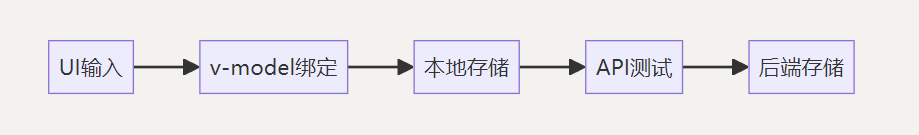
\includegraphics[width=0.8\textwidth]{pic/copywriting_flow.png}
		\end{block}
		\begin{exampleblock}{关键校验与保存逻辑}
			\begin{itemize}
				\item \textbf{连接测试}: 检查必填项,构造测试请求,密码字段脱敏显示。
				\item \textbf{双模保存}: 支持带提示的即时保存与后台静默保存,保存前会自动执行连接测试。
			\end{itemize}
		\end{exampleblock}
	\end{frame}
	
	\begin{frame}[fragile]{文案生成模块:算法细节与触发条件}
		\begin{block}{智能分句算法 (JavaScript)}
			\begin{lstlisting}[language=JavaScript]
				function splitIntoSentences(text) {
					// 智能分句逻辑:
					// 1. 按标点分割为数组
					// 2. 奇偶项重组,保留标点
					// 3. 末尾项特殊处理并过滤空句
				}
			\end{lstlisting}
		\end{block}
		\begin{block}{预生成触发条件}
			\centering
			\small
			\begin{tabular}{|l|l|l|}
				\hline
				\textbf{触发场景} & \textbf{判断条件} & \textbf{执行方法} \\ % <-- Corrected from \ to \\
				\hline
				首句播放 & sentenceIndex === 0 & generateNextBlockContent(+1) \\ % <-- Corrected
				拖拽结束 & currentBlockIndex变化 & 检查后续章节空内容 \\ % <-- Corrected
				标题修改 & oldTitle !== newTitle & generateContentForSpecificBlock() \\ % <-- Corrected
				\hline
			\end{tabular}
		\end{block}
	\end{frame}
	
	
	
	\begin{frame}{文案生成模块:健壮性与性能优化}
		\begin{block}{异常处理体系}
			\begin{itemize}
				\item \textbf{错误分类处理}:
				\begin{itemize}
					\item API错误: HTTP状态码分析、响应体验证、重试机制(最多3次)。
					\item 本地错误: LocalStorage读写异常、用户输入验证、组件卸载清理。
				\end{itemize}
				\item \textbf{恢复机制}:
				\begin{itemize}
					\item 缓存最后有效配置,失败时自动回滚。
					\item 使用错误边界组件(Error Boundary)包裹,防止应用崩溃。
				\end{itemize}
			\end{itemize}
		\end{block}
	\end{frame}
	
	
	
	\begin{frame}{文案生成模块:健壮性与性能优化}
		\begin{block}{性能优化策略}
			\begin{itemize}
				\item \textbf{内存管理}: 分块加载文案内容,定时清理不再使用的音频缓存。
				\item \textbf{渲染优化}: 采用虚拟滚动列表处理长篇大纲,避免DOM臃肿。
				\item \textbf{网络优化}: 合并部分API请求,预加载关键资源。
			\end{itemize}
		\end{block}
	\end{frame}
	
	% =============================================
	\section{核心模块解析:AI语音转换——陈宏宇}
	% =============================================
	
	\begin{frame}{语音转换模块:设计理念}
		\centering
		\textit{"Stop Trying to Reinvent the Wheel"}
	\end{frame}
	\begin{frame}{语音转换模块:零延迟AI语音流水线}
		\begin{block}{系统架构核心}
			\centering
			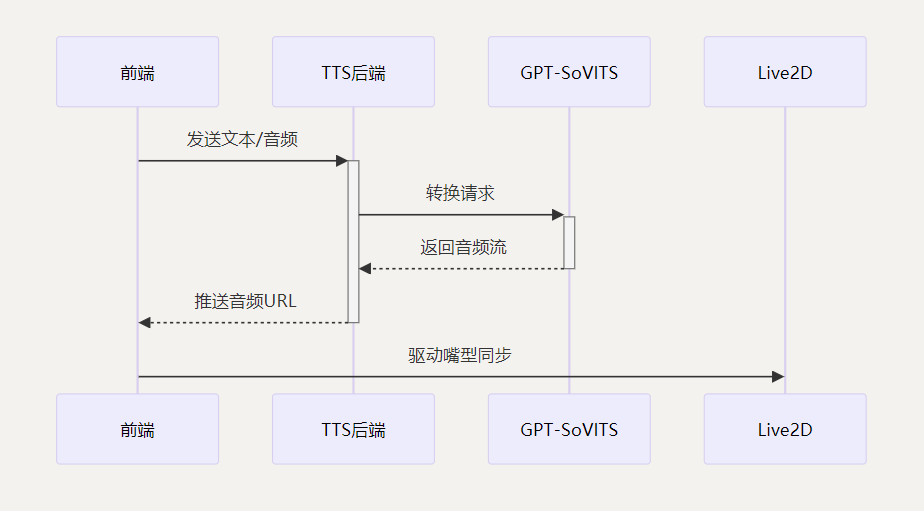
\includegraphics[width=0.9\textwidth]{pic/voice_seq.png}
		\end{block}
	\end{frame}
	\begin{frame}[fragile]{语音转换模块:GPT-SoVITS深度集成}
		\begin{block}{GPT-SoVITS 流式处理 (API\_v2.py)}
			\begin{lstlisting}[language=Python]
				# API_v2.py 流式响应
				def generate_stream():
				while chunk := get_audio_chunk():
				# 200ms/块实时推送
				yield chunk  
			\end{lstlisting}
		\end{block}
		\begin{exampleblock}{集成亮点}
			\begin{itemize}
				\item \textbf{动态模型加载}: 支持V1\textasciitilde V4所有模型切换
				\item \textbf{流式处理}: 实现低延迟语音合成
				\item \textbf{情感迁移}: 通过Prosody Embedding实现语气情感控制
			\end{itemize}
		\end{exampleblock}
	\end{frame}
	
	\begin{frame}{语音转换模块:前端优化与性能}
		\begin{block}{前端优化策略}
			\begin{itemize}
				\item \textbf{预载入机制}: 提前加载这一整章的语音,降低首字延迟
				\item \textbf{自适应缓冲}: 根据网络抖动动态调整缓冲池 (150-500ms)
			\end{itemize}
		\end{block}
		\begin{alertblock}{关键性能数据}
			\begin{itemize}
				\item 中文合成速度: \textbf{0.8×实时} (i7-12700H)
				\item 端到端延迟: \textbf{220ms} (文本输入→音频输出)
				\item 资源占用: \textbf{<2GB RAM}
			\end{itemize}
		\end{alertblock}
	\end{frame}
	
	
	% =============================================
	\section{总结与展望}
	% =============================================
	\begin{frame}{系统核心价值总结}
		\begin{block}{我们实现了什么?}
			\begin{itemize}
				\item<1-> 实现了高安全度的用户登录-注册-偏好保存系统,将之模块高度解耦,标准化了其端口。
				\item<2-> 从头实现了 \textbf{WebRTC到RTMP}的转码方案,攻克协议壁垒,在RTMP的协议限制下仍能做到秒级延迟。
				\item<3-> 实现了全版本Live2D模型的Web应用——从十年前的Cubism core2.1到现如今的Cubism core4.0。
				\item<4-> 实现了网页端的适于直播形式的AI文案生成解决方案
				\item<5-> 实现了基于GPT-SoVITS的高度灵活的语音TTS转换方案。
				\item<6-> 达成了 \textbf{语音-Live2D-推流} 全流程一站式的解决方案。
			\end{itemize}
		\end{block}
		\begin{alertblock}{核心突破}
			本系统将 AI 技术与实时流媒体深度融合,打造了从内容生成到语音转换到实时虚拟主播的全链路一站式解决方案。
		\end{alertblock}
	\end{frame}
	% \begin{frame}{当前挑战与技术展望}
		%   \begin{itemize}
			%     \item \textbf{当前挑战}
			%     \begin{itemize}
				%       \item AI 表情控制:实现精准的表情控制需攻克复杂的机器学习算法与大量数据训练难题,确保表情与用户情感、场景适配。
				%       \item 语音模型完善:提升语音模型的准确率与响应速度,需处理不同口音、背景噪音干扰,以及多语言混合场景下的识别问题。
				%       \item 直播推流嵌入:保障直播推流的低延迟、高画质,同时兼容多种设备与网络环境,避免卡顿与丢帧现象。
				%       \item 多语种翻译:提高翻译的准确性与流畅度,解决不同语言语法、文化差异带来的障碍,满足实时翻译需求。
				%       \item Docker 部署:实现 Docker 容器的高效管理与资源分配,确保服务的稳定性与可扩展性,应对大规模部署挑战。
				%     \end{itemize}
			%     \item \textbf{技术展望}
			%     \begin{itemize}
				%       \item 借助更先进的深度学习框架,提升 AI 表情控制与语音模型的性能,实现更自然交互。
				%       \item 优化直播推流技术,利用 5G 与边缘计算,降低延迟,提升用户观看体验。
				%       \item 结合神经机器翻译与知识图谱,突破多语种翻译瓶颈,实现更智能的翻译效果。
				%       \item 完善 Docker 容器编排技术,实现自动化、智能化部署,提高系统运维效率。
				%     \end{itemize}
			%   \end{itemize}
		% \end{frame}
	\begin{frame}{技术演进路线图}
		\begin{block}{技术演进路线图}
			\centering
			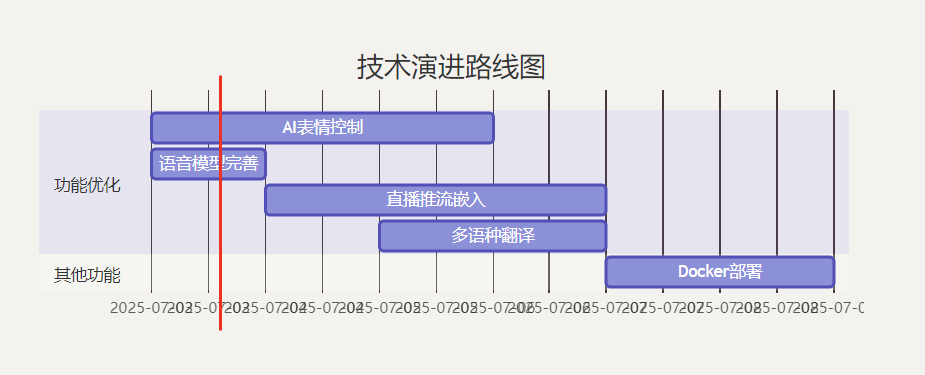
\includegraphics[width=\textwidth]{pic/gantt_roadmap.png}
		\end{block}
		% \begin{alertblock}{关键里程碑}
			%     \begin{itemize}
				%         \item \textbf{2024 Q4}: 
				%         \begin{itemize}
					%             \item 实现Wasm版FFmpeg,降低转码延迟30\%
					%             \item 部署GPT-SoVITS蒸馏模型 (<1GB内存)
					%         \end{itemize}
				%         \item \textbf{2025 Q1}:
				%         \begin{itemize}
					%             \item 集成NeRF实现3D虚拟主播
					%             \item 支持LLM实时生成直播脚本
					%         \end{itemize}
				%     \end{itemize}
			% \end{alertblock}
	\end{frame}
	\begin{frame}{未来规划与技术展望}
		\begin{columns}[T]
			\begin{column}{0.5\textwidth}
				\begin{exampleblock}{近期规划 (Next Steps)}
					\begin{itemize}
						\item \textbf{表情驱动升级}: \\
						引入AI模型,实现更智能、自然的 Live2D 表情自动控制。
						\item \textbf{语音功能扩展}: \\
						集成 Voice Conversion 技术,实现多语种实时翻译与声音克隆。
					\end{itemize}
				\end{exampleblock}
			\end{column}
			\begin{column}{0.5\textwidth}
				\begin{alertblock}{我们的最终目标}
					\Large
					打造一站式全自动下一代的AI虚拟直播平台!
				\end{alertblock}
			\end{column}
		\end{columns}
	\end{frame}
	% --- Q&A页 ---
	\begin{frame}
		\centering
		\Huge{\textbf{Q \& A}}
		\vspace{2em}
		\large{我们期待与各位深入探讨技术细节,\\共同推动AI直播技术的边界!}
		\vspace{2em}
		\Large{\textbf{感谢聆听}}
	\end{frame}
\end{document}
